\documentclass[10pt, a4paper]{article}\usepackage[]{graphicx}\usepackage[]{color}
% maxwidth is the original width if it is less than linewidth
% otherwise use linewidth (to make sure the graphics do not exceed the margin)
\makeatletter
\def\maxwidth{ %
  \ifdim\Gin@nat@width>\linewidth
    \linewidth
  \else
    \Gin@nat@width
  \fi
}
\makeatother

\definecolor{fgcolor}{rgb}{0.345, 0.345, 0.345}
\newcommand{\hlnum}[1]{\textcolor[rgb]{0.686,0.059,0.569}{#1}}%
\newcommand{\hlstr}[1]{\textcolor[rgb]{0.192,0.494,0.8}{#1}}%
\newcommand{\hlcom}[1]{\textcolor[rgb]{0.678,0.584,0.686}{\textit{#1}}}%
\newcommand{\hlopt}[1]{\textcolor[rgb]{0,0,0}{#1}}%
\newcommand{\hlstd}[1]{\textcolor[rgb]{0.345,0.345,0.345}{#1}}%
\newcommand{\hlkwa}[1]{\textcolor[rgb]{0.161,0.373,0.58}{\textbf{#1}}}%
\newcommand{\hlkwb}[1]{\textcolor[rgb]{0.69,0.353,0.396}{#1}}%
\newcommand{\hlkwc}[1]{\textcolor[rgb]{0.333,0.667,0.333}{#1}}%
\newcommand{\hlkwd}[1]{\textcolor[rgb]{0.737,0.353,0.396}{\textbf{#1}}}%
\let\hlipl\hlkwb

\usepackage{framed}
\makeatletter
\newenvironment{kframe}{%
 \def\at@end@of@kframe{}%
 \ifinner\ifhmode%
  \def\at@end@of@kframe{\end{minipage}}%
  \begin{minipage}{\columnwidth}%
 \fi\fi%
 \def\FrameCommand##1{\hskip\@totalleftmargin \hskip-\fboxsep
 \colorbox{shadecolor}{##1}\hskip-\fboxsep
     % There is no \\@totalrightmargin, so:
     \hskip-\linewidth \hskip-\@totalleftmargin \hskip\columnwidth}%
 \MakeFramed {\advance\hsize-\width
   \@totalleftmargin\z@ \linewidth\hsize
   \@setminipage}}%
 {\par\unskip\endMakeFramed%
 \at@end@of@kframe}
\makeatother

\definecolor{shadecolor}{rgb}{.97, .97, .97}
\definecolor{messagecolor}{rgb}{0, 0, 0}
\definecolor{warningcolor}{rgb}{1, 0, 1}
\definecolor{errorcolor}{rgb}{1, 0, 0}
\newenvironment{knitrout}{}{} % an empty environment to be redefined in TeX

\usepackage{alltt}
    \pagestyle{empty}
    \renewcommand{\baselinestretch}{1.5}
    \usepackage[english]{babel}
 
\usepackage[top=2.2cm,bottom=2.2cm, left = 2.1cm, right = 2.1cm]{geometry}
\usepackage{latexsym}
\usepackage{graphicx}
\usepackage{amsmath, amssymb}
\usepackage[utf8]{inputenc}
\usepackage{mathpazo}
\usepackage{geometry}
\usepackage{amsfonts}
\usepackage{ifsym}
\usepackage{booktabs}
\usepackage{enumerate}
\usepackage{a4wide}
\usepackage{float}
\usepackage{dsfont}
\usepackage{hhline}
\usepackage{lscape}
\usepackage{stmaryrd}
\usepackage{paralist}
%\usepackage[utf8]{inputenc}
\usepackage{fancyhdr}
\usepackage{nicefrac}


\usepackage[usenames,x11names]{xcolor} % Die Optionen definieren zusätzliche Farben (siehe Dokumentation)
\usepackage{graphicx}
\usepackage{subfigure}
% Tikz zeug
\usepackage{tikz}
\usepackage{tkz-tab}
\newcommand{\widebar}{\overline}


%\input{definitionen}

\newfont{\suet}{suet14}
\DeclareTextFontCommand{\textsuet}{\suet}



\newcommand{\Var}{\text{Var}}
\newcommand{\Ew}{\mathbb{E}}
\newcommand{\med}{\text{med}}
\newcommand{\MSE}{\text{MSE}}
\newcommand{\Bias}{\text{Bias}}
\newcommand{\A}{\mathcal{A}}
\renewcommand{\O}{\Omega}
\newcommand{\R}{\mathbb{R}}
\newcommand{\N}{\mathbb{N}}
\newcommand{\Borell}{\mathfrak{B}}
\renewcommand{\P}{\mathcal{P}}
\newcommand{\vt}{\vartheta}
\renewcommand{\le}{\leqslant} % ich finde Kleinergleich mit schrägen Strich schöner
\renewcommand{\ge}{\geqslant}

%-- charakteristische-Funktion-/Indikatorfunktion-Eins '\ind'
\usepackage{silence}
\WarningFilter{latexfont}{Size substitutions with differences}
\WarningFilter{latexfont}{Font shape `U/bbold/m/n' in size}
\DeclareSymbolFont{bbold}{U}{bbold}{m}{n}
\DeclareSymbolFontAlphabet{\mathbbold}{bbold}
\newcommand{\ind}{\mathbbold{1}} 

    \setlength{\textwidth}{15cm}
\setlength{\oddsidemargin}{0.5cm}

\setlength{\parskip}{2ex plus0.5ex minus0.5ex}
\setlength{\parindent}{0em}
\renewcommand{\labelenumi}{\alph{enumi})}
\renewcommand{\vt}{\vartheta}
\newcommand{\E}{\mathbb{E}}
\newcommand{\V}{\mathbb{V}\text{ar}}
\newcommand{\C}{\mathbb{C}\text{ov}}
\renewcommand{\P}{\mathbb{P}}
\IfFileExists{upquote.sty}{\usepackage{upquote}}{}
\begin{document}
	
	



\subsection*{Parameter Estimation of a Mixture Distribution}
Let $X_1,\dots,X_n$ be a stationary time series with extremal index $\theta\in (0,1]$ (see Beirlant et al, 2004) and $W_1,\dots,W_n$ iid, heavy-tailed waiting times. We can show that the limiting distribution of the excess waiting times with threshold $u_n$ ($u_n \rightarrow x_R$) is a mixture distribution out of the dirac measure at point zero and the Mittag-Leffler distribution $ML(\beta,\theta^{-1/\beta})$, $\beta \in (0,1]$, with weights $(1-\theta,\theta)$ :
\begin{align} \label{eq3}
	\mathbb{P}_{\beta,\theta}:=(1-\theta)\delta_0+\theta \cdot ML(\beta,\theta^{-1/\beta}).
\end{align}
We want to estimate the two unknown parameters $\beta$ and $\theta$ with the method of moments. But since the ML-distribution does not have finite moments we have a look at the fractional moments. Let $q \in (0,1)$. The $q$-th fractional moment of a $ML(\beta,\gamma)$-distributed random variable $Y$ is:
\begin{align}
\mathbb{E}(Y^q)=\frac{ q \cdot \pi \cdot  \gamma^q}{\beta \cdot \Gamma(1-q)\sin(\frac{q \cdot \pi}{\beta})}, \qquad \text{for } 0 < q < \beta
\end{align}
(Cahoy, 2013). 
Then the $q$-th fractional moment of $T \sim \mathbb{P}_{\beta,\theta}$ is
\begin{align} \label{eq1}
m_q:=m_q(T):&=\mathbb{E}(T^q) = (1-\theta)\mathbb{E}(Y^q)+\theta\mathbb{E}(X^q) = \theta\mathbb{E}(X^q) \\
&= \theta^{\frac{\beta-q}{\beta}} \cdot \frac{ q \cdot \pi  }{\beta \cdot \Gamma(1-q)\sin(\frac{q \cdot \pi}{\beta})} \nonumber
\end{align}
with $Y \sim \delta_0$ and $X \sim ML(\beta,\theta^{-1/\beta})$, $q<\beta$.
The empirical $q$-th fractional moment $\hat{m}_q=\frac{1}{n}\sum_{i=1}^{n}T_i^q$, $T_1,\dots,T_n \overset{iid}{\sim} \mathbb{P}_{\beta,\theta}$, is an unbiased estimator of $m_q$ and for $2q < \beta$ the estimator $\hat{m}_q$ is consistent in mean square:
\begin{align}
	\text{Var}(\hat{m}_q)
	&=\mathbb{E}(\hat{m}_q^2)-\mathbb{E}(\hat{m}_q)^2 \\ \nonumber
	&= \frac{1}{n^2}\mathbb{E}\left( \sum_{i \neq j} T_i^q T_j^q + \sum_{i=1}^{n} T_i^{2q} \right) - m_q^2 \\ \nonumber
	&= \frac{1}{n^2}\left(  n(n-1) \mathbb{E}(T_1^q)^2 + n \mathbb{E}(T_1^{2q}) \right) - m_q^2 \\ \nonumber
	&= \frac{n-1}{n} m_q^2 + \frac{1}{n} m_{2q} - m_q^2 \overset{n \to \infty}{\longrightarrow} 0. 
\end{align}
Since $\lim\limits_{x \to 0}\frac{\sin(x\pi)}{x\pi} = 1$ (easily shown by using L'Hopital's rule) and $\Gamma(1)=1$ it follows 
\begin{align} \label{eq2}
	\lim\limits_{q \to 0} m_q = \theta.
\end{align}
By solving (\ref{eq1}) for $\theta$ and using the empirical fractional moment $\hat{m}_q$, we get an estimator $\hat{\theta}_q(\beta)$ depending on $\beta$:
\begin{align}
	\hat{\theta}_q(\beta)=\left[ \frac{\beta \cdot \Gamma(1-q)\sin(\frac{q \cdot \pi}{\beta})}{q \cdot \pi} \cdot \widehat{m}_q \right]^{\frac{\beta}{\beta-q}}
\end{align}
Therefore, we have to estimate $\beta$ first by calculating the root of $\hat{\theta}_{q_1}(\beta)-\hat{\theta}_{q_2}(\beta)$ on $(\max(q_1,q_2),1]$ (we choose $\max(q_1,q_2)$ as the lower interval limit because $\beta>q_1,q_2$ has to be fulfilled, otherwise the fractional moments don't exist). 
It is important to choose the fractions $q_1$ and $q_2$ small enough (smaller than the (unknown) $\beta$) otherwise we can't find $\beta$ by calculating the root of $\hat{\theta}_{q_1}(\beta)-\hat{\theta}_{q_2}(\beta)$ because $\beta \notin (\max(q_1,q_2),1]$ for $\beta \le q_1,q_2$. $\hat{\theta}_q(\beta)$ is not unbiased but for smaller $q$ the bias gets smaller because of (\ref{eq2}).

\begin{figure} 
\begin{knitrout}
\definecolor{shadecolor}{rgb}{0.969, 0.969, 0.969}\color{fgcolor}

{\centering 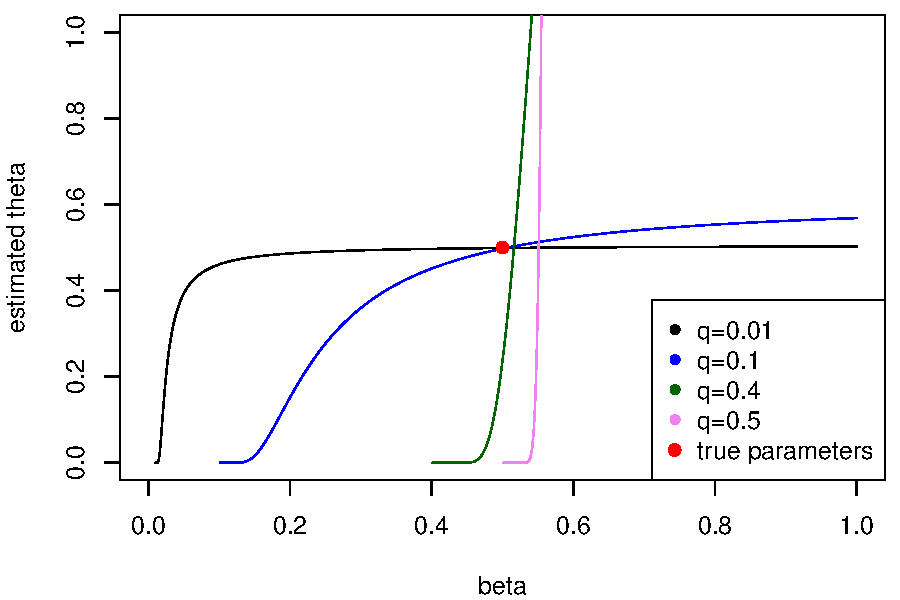
\includegraphics[width=.6\linewidth]{figure/minimal-plot1_-1} 

}



\end{knitrout}
\vspace{-0.4cm}
\caption{Estimation $\hat{\theta}_q(\beta)$ depending on $\beta$ for various fractions $q$. It is based on $n=10000$ $\mathbb{P}_{0.5,0.5}$-distributed data.}
\label{fig1}
\end{figure}
Figure \ref{fig1} shows $\hat{\theta}_q(\beta)$ depending on $\beta$ for various fractions $q$. We can see that the curves of lower fractions $q$ intersect the true parameter while the curve of $p=0.5=\beta$ doesn't. As well we can see that for small fraction $q$ the estimator $\hat{\theta}_q(\beta)$ is less dependend of $\beta$.
\\
Now we look how it works with \texttt{R}:
\begin{knitrout}
\definecolor{shadecolor}{rgb}{0.969, 0.969, 0.969}\color{fgcolor}\begin{kframe}
\begin{alltt}
\hlkwd{set.seed}\hlstd{(}\hlnum{2345}\hlstd{)}
\hlcom{## chosen parameters:}
\hlcom{# 1) true parameters}
\hlstd{beta} \hlkwb{<-} \hlnum{0.5}
\hlstd{theta} \hlkwb{<-} \hlnum{0.5}
\hlcom{# 2) random sample}
\hlstd{n} \hlkwb{<-} \hlnum{10000}                                   \hlcom{# sample size}
\hlcom{# 3) fractions}
\hlstd{q1} \hlkwb{<-} \hlnum{0.01}
\hlstd{q2} \hlkwb{<-} \hlnum{0.05}
\hlcom{## sample:}
\hlstd{prob} \hlkwb{<-} \hlkwd{sample}\hlstd{(} \hlkwd{c}\hlstd{(}\hlnum{0}\hlstd{,}\hlnum{1}\hlstd{) ,} \hlkwc{size} \hlstd{= n ,} \hlkwc{replace} \hlstd{= T ,} \hlkwc{prob} \hlstd{=} \hlkwd{c}\hlstd{(}\hlnum{1}\hlopt{-}\hlstd{theta , theta))}
\hlcom{# we need the R-package 'MittagLeffleR' to sample ML-distributed values:}
\hlcom{# install.packages("MittagLeffleR") }
\hlstd{daten} \hlkwb{<-} \hlkwd{sapply}\hlstd{(prob ,}                       \hlcom{# sample}
                \hlkwa{function}\hlstd{(}\hlkwc{x}\hlstd{)\{} \hlkwd{ifelse}\hlstd{( x} \hlopt{==} \hlnum{0} \hlstd{,} \hlkwd{return}\hlstd{(}\hlnum{0}\hlstd{) ,}
                        \hlkwd{return}\hlstd{( MittagLeffleR}\hlopt{::}\hlkwd{rml}\hlstd{(}\hlnum{1} \hlstd{,} \hlkwc{tail} \hlstd{= beta ,}
                        \hlkwc{scale} \hlstd{= theta}\hlopt{^}\hlstd{(}\hlopt{-}\hlnum{1}\hlopt{/}\hlstd{beta))}
                        \hlstd{) ) \} )}
\hlcom{## functions:}
\hlstd{fct_empfracmom} \hlkwb{<-} \hlkwa{function}\hlstd{(} \hlkwc{q} \hlstd{,} \hlkwc{data} \hlstd{)\{}       \hlcom{# emp. frac. moment}
                \hlstd{r} \hlkwb{<-} \hlnum{1}\hlopt{/}\hlstd{(}\hlkwd{length}\hlstd{(data))}\hlopt{*}\hlkwd{sum}\hlstd{(data}\hlopt{^}\hlstd{q)}
                \hlkwd{return}\hlstd{(r)       \}}
\hlstd{fct_theta} \hlkwb{<-} \hlkwa{function}\hlstd{(} \hlkwc{beta} \hlstd{,} \hlkwc{q} \hlstd{,} \hlkwc{data} \hlstd{)\{}     \hlcom{# estimator for theta}
                \hlstd{r} \hlkwb{<-} \hlstd{( ( beta}\hlopt{*}\hlkwd{gamma}\hlstd{(}\hlnum{1}\hlopt{-}\hlstd{q)}\hlopt{*}\hlkwd{sin}\hlstd{(pi}\hlopt{*}\hlstd{q}\hlopt{/}\hlstd{beta) )}\hlopt{/}\hlstd{( q}\hlopt{*}\hlstd{pi )}\hlopt{*}
                \hlkwd{fct_empfracmom}\hlstd{(q , data) )}\hlopt{^}\hlstd{(beta}\hlopt{/}\hlstd{(beta}\hlopt{-}\hlstd{q))}
                \hlkwd{return}\hlstd{(r)               \}}
\hlstd{fct_root} \hlkwb{<-} \hlkwa{function}\hlstd{(} \hlkwc{beta} \hlstd{,} \hlkwc{q1} \hlstd{,} \hlkwc{q2} \hlstd{,} \hlkwc{data}\hlstd{)\{}
                \hlstd{r} \hlkwb{<-} \hlkwd{fct_theta}\hlstd{( beta , q1 , data)} \hlopt{-} \hlkwd{fct_theta}\hlstd{( beta , q2 , data)}
                \hlkwd{return}\hlstd{(r)                  \}}
\hlstd{fct_beta} \hlkwb{<-} \hlkwa{function}\hlstd{(}\hlkwc{q1} \hlstd{,} \hlkwc{q2} \hlstd{,} \hlkwc{data}\hlstd{)\{}         \hlcom{# estimator for beta}
                \hlstd{r} \hlkwb{<-} \hlkwd{uniroot}\hlstd{(fct_root ,} \hlkwd{c}\hlstd{(}\hlkwd{max}\hlstd{(q1,q2)}\hlopt{+}\hlnum{0.001}\hlstd{,}\hlnum{1}\hlstd{) ,} \hlkwc{q1} \hlstd{= q1 ,}
                \hlkwc{q2} \hlstd{= q2 ,} \hlkwc{data} \hlstd{= data)}
                \hlkwd{return}\hlstd{(r}\hlopt{$}\hlstd{root)      \}}
\hlcom{## estimating beta and theta}
\hlcom{# estimating beta by calculating the root:}
\hlstd{beta_hat1} \hlkwb{<-} \hlkwd{fct_beta}\hlstd{(}\hlkwc{q1}\hlstd{=q1 ,} \hlkwc{q2}\hlstd{=q2 ,} \hlkwc{data} \hlstd{= daten); beta_hat1}
\end{alltt}
\begin{verbatim}
## [1] 0.4992572
\end{verbatim}
\begin{alltt}
\hlcom{# estimating theta by using beta_hat1}
\hlstd{theta_hat11} \hlkwb{<-} \hlkwd{fct_theta}\hlstd{(}\hlkwc{beta} \hlstd{= beta_hat1 ,} \hlkwc{q}\hlstd{=q1 ,} \hlkwc{data} \hlstd{= daten); theta_hat11}
\end{alltt}
\begin{verbatim}
## [1] 0.5020829
\end{verbatim}
\begin{alltt}
\hlstd{theta_hat12} \hlkwb{<-} \hlkwd{fct_theta}\hlstd{(}\hlkwc{beta} \hlstd{= beta_hat1 ,} \hlkwc{q}\hlstd{=q2 ,} \hlkwc{data} \hlstd{= daten); theta_hat12}
\end{alltt}
\begin{verbatim}
## [1] 0.5020837
\end{verbatim}
\begin{alltt}
\hlcom{# error:}
\hlkwd{abs}\hlstd{(beta}\hlopt{-}\hlstd{beta_hat1);} \hlkwd{abs}\hlstd{(theta}\hlopt{-}\hlstd{theta_hat11);} \hlkwd{abs}\hlstd{(theta}\hlopt{-}\hlstd{theta_hat12)}
\end{alltt}
\begin{verbatim}
## [1] 0.0007427727
## [1] 0.00208289
## [1] 0.002083718
\end{verbatim}
\begin{alltt}
\hlcom{## -> it works}

\hlcom{# estimating theta by calculating the q-th emp. frac. moment with q very small: }
\hlstd{theta_hat2} \hlkwb{<-} \hlkwd{fct_empfracmom}\hlstd{(}\hlnum{10}\hlopt{^}\hlstd{\{}\hlopt{-}\hlnum{6}\hlstd{\} ,} \hlkwc{data}\hlstd{=daten); theta_hat2}
\end{alltt}
\begin{verbatim}
## [1] 0.5021004
\end{verbatim}
\begin{alltt}
\hlstd{beta_hat2} \hlkwb{<-} \hlkwd{uniroot}\hlstd{(}\hlkwa{function}\hlstd{(}\hlkwc{x}\hlstd{)\{}\hlkwd{fct_theta}\hlstd{(x ,} \hlkwc{q}\hlstd{=q1 ,} \hlkwc{data}\hlstd{=daten)}\hlopt{-}\hlstd{theta_hat2\} ,}
\hlkwc{interval} \hlstd{=} \hlkwd{c}\hlstd{(q1,}\hlnum{1}\hlstd{))}\hlopt{$}\hlstd{root; beta_hat2}
\end{alltt}
\begin{verbatim}
## [1] 0.5003904
\end{verbatim}
\begin{alltt}
\hlkwd{abs}\hlstd{(beta}\hlopt{-}\hlstd{beta_hat2);} \hlkwd{abs}\hlstd{(theta}\hlopt{-}\hlstd{theta_hat2)}
\end{alltt}
\begin{verbatim}
## [1] 0.0003903841
## [1] 0.002100401
\end{verbatim}
\begin{alltt}
\hlcom{## -> works as well; }
\hlcom{## -> unsolved problem: which fraction q is small enough }
\hlcom{##    to estimate theta reliably?}
\end{alltt}
\end{kframe}
\end{knitrout}
\end{document}


